\documentclass{beamer}
\usetheme{Madrid}
\usepackage{amsmath, amssymb, listings, xcolor}
\usepackage{tikz}
\usetikzlibrary{positioning, arrows.meta, shapes}

% ── Global TikZ styles ────────────────────────────────────────────────────────
\tikzset{
  % Large stage box for the pipeline block diagram
  stage/.style={
    draw, rectangle,
    minimum width=1.40cm, minimum height=0.65cm,
    fill=blue!25, font=\small\bfseries, align=center
  },
  % Normal pipeline-stage cell in timing diagrams (blue)
  blk/.style={
    draw, rectangle,
    minimum width=0.60cm, minimum height=0.38cm,
    fill=blue!25, font=\tiny\bfseries,
    inner sep=0pt, align=center
  },
  % Stall cell (red bubble) in timing diagrams
  stl/.style={
    draw, rectangle,
    minimum width=0.60cm, minimum height=0.38cm,
    fill=red!30, font=\tiny\bfseries,
    inner sep=0pt, align=center
  },
  % Invisible spacer cell (anchors bounding box)
  emp/.style={minimum width=0.60cm, minimum height=0.38cm},
  % Hardware pipeline arrow
  harr/.style={-{Stealth}, thick},
  % Forwarding bypass arrow
  fwdarr/.style={-{Stealth}, thick, dashed, green!60!black},
}
% ─────────────────────────────────────────────────────────────────────────────

\title{Understanding Pipelining Hazards}
\subtitle{BLG 483E -- Artificial Intelligence}
\author{salihsefer36}
\date{\today}

\begin{document}

% ═════════════════════════════════════════════════════════════════════════════
% Slide 1 — Title
% ═════════════════════════════════════════════════════════════════════════════
\begin{frame}
  \titlepage
\end{frame}

% ═════════════════════════════════════════════════════════════════════════════
% Slide 2 — Introduction to CPU Pipelining  [v2 — unchanged]
% ═════════════════════════════════════════════════════════════════════════════
\begin{frame}{Introduction to CPU Pipelining}
  \textit{Think of a restaurant: one waiter takes orders, one chef cooks,
  another plates, another serves. If one person did everything per customer,
  the restaurant would serve one table at a time. A CPU pipeline works
  exactly the same way.}

  \medskip
  \begin{itemize}
    \item A pipeline splits every instruction into 5 stages that run
          \textbf{simultaneously} for different instructions:
          \textbf{IF} (fetch), \textbf{ID} (decode), \textbf{EX} (execute),
          \textbf{MEM} (memory), \textbf{WB} (write result).
    \item When the assembly line runs smoothly, the CPU completes roughly
          one instruction per clock cycle (instead of one every 5 cycles).
    \item A \textbf{hazard} is anything that breaks the smooth flow ---
          a conflict that forces a stage to wait or throw away work.
    \item Hazards come in three flavours: \textbf{data}, \textbf{structural},
          and \textbf{control}.
  \end{itemize}
\end{frame}

% ═════════════════════════════════════════════════════════════════════════════
% Slide 3 — NEW: The 5-Stage Pipeline  [TikZ Diagram 1]
% ═════════════════════════════════════════════════════════════════════════════
\begin{frame}{The 5-Stage Pipeline}

  % ── Block diagram: IF → ID → EX → MEM → WB ─────────────────────────────
  \begin{center}
  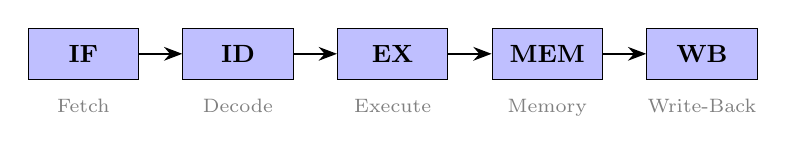
\begin{tikzpicture}
    \node[stage]                      (IF)  {IF};
    \node[stage, right=0.55cm of IF]  (ID)  {ID};
    \node[stage, right=0.55cm of ID]  (EX)  {EX};
    \node[stage, right=0.55cm of EX]  (MEM) {MEM};
    \node[stage, right=0.55cm of MEM] (WB)  {WB};

    \draw[harr] (IF)--(ID);
    \draw[harr] (ID)--(EX);
    \draw[harr] (EX)--(MEM);
    \draw[harr] (MEM)--(WB);

    \node[below=0.12cm of IF,  font=\scriptsize, text=gray] {Fetch};
    \node[below=0.12cm of ID,  font=\scriptsize, text=gray] {Decode};
    \node[below=0.12cm of EX,  font=\scriptsize, text=gray] {Execute};
    \node[below=0.12cm of MEM, font=\scriptsize, text=gray] {Memory};
    \node[below=0.12cm of WB,  font=\scriptsize, text=gray] {Write-Back};
  \end{tikzpicture}
  \end{center}

  \smallskip
  \begin{itemize}
    \item \textbf{IF} fetches the raw binary instruction from the instruction cache.
    \item \textbf{ID} decodes opcodes and reads source-register values.
    \item \textbf{EX} runs the ALU operation (add, subtract, address compute).
    \item \textbf{MEM} reads from or writes to the data cache.
    \item \textbf{WB} commits the computed value to the destination register.
  \end{itemize}

  \begin{center}
    \scriptsize In a \emph{hazard-free} pipeline a new instruction enters
    IF every cycle. \textbf{Hazards break this ideal.}
  \end{center}
\end{frame}

% ═════════════════════════════════════════════════════════════════════════════
% Slide 4 — Data Hazards: Types  [v2 — unchanged]
% ═════════════════════════════════════════════════════════════════════════════
\begin{frame}{Data Hazards --- Types}
  \textit{Imagine a relay race where runner B must grab the baton from runner A
  before sprinting. If B takes off before A arrives, the handoff fails.
  Data hazards are exactly that: one instruction needs a value the previous
  one has not finished computing yet.}

  \medskip
  \begin{itemize}
    \item \textbf{RAW} (Read-After-Write, ``true dependence''): the most common
          type. Instruction B tries to read a register before instruction A has
          written its result into it. \textit{Runner B starts before the baton
          arrives.}
    \item \textbf{WAR} (Write-After-Read, ``anti-dependence''): B wants to
          overwrite a register that A is still reading. \textit{Chef B wants to
          clean the pan that chef A is still using.}
    \item \textbf{WAW} (Write-After-Write, ``output dependence''): two
          instructions both write the same register; the second write must
          ``win''. \textit{Two workers submit the same report; only the later
          version should be filed.}
  \end{itemize}
\end{frame}

% ═════════════════════════════════════════════════════════════════════════════
% Slide 5 — Data Hazards: Detection & Mitigation  [v2 — unchanged]
% ═════════════════════════════════════════════════════════════════════════════
\begin{frame}{Data Hazards --- Detection \& Mitigation}
  \textit{Think of a traffic officer watching an intersection. When two cars
  are about to collide, the officer either holds one back (stall) or waves it
  through a special shortcut lane (forwarding).}

  \medskip
  \begin{itemize}
    \item \textbf{Detection:} A hazard detection unit (``the traffic officer'')
          checks the pipeline registers (ID/EX, EX/MEM, MEM/WB) every cycle
          to spot conflicts before they cause wrong results.
    \item \textbf{Stall (interlock):} Freeze the fetch and decode stages,
          insert a bubble (an empty ``do nothing'' slot) --- like holding a car
          at a red light for one cycle.
    \item \textbf{Forwarding (bypassing):} Route the computed result directly
          from one pipeline stage to the next instruction's input, skipping the
          detour through the register file. Eliminates most RAW stalls completely.
    \item \textbf{Load-use exception:} When instruction A loads from memory and
          B immediately needs that value, forwarding still cannot help --- one
          stall cycle is unavoidable.
  \end{itemize}
\end{frame}

% ═════════════════════════════════════════════════════════════════════════════
% Slide 6 — NEW: Worked Example — RAW Hazard & Forwarding  [TikZ Diagram 2 + tabular]
% ═════════════════════════════════════════════════════════════════════════════
\begin{frame}{Worked Example: RAW Hazard \& Forwarding}

  \texttt{\scriptsize I1:~ADD~R1,R2,R3} \qquad
  \texttt{\scriptsize I2:~SUB~R4,\textcolor{red}{R1},R5}
  \;{\scriptsize --- I2 reads R1 produced by I1 (\textbf{RAW} dependence)}

  \smallskip
  \begin{columns}[T]

    % ── Left column: Without Forwarding (8 cycles, 2 red stalls) ────────────
    \begin{column}{0.50\textwidth}
      \centering{\small\textbf{Without Forwarding}}
      \begin{center}
      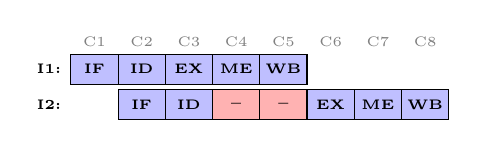
\begin{tikzpicture}
        % Cycle-number header row
        \foreach \idx/\cx in
          {1/0.30, 2/0.90, 3/1.50, 4/2.10, 5/2.70, 6/3.30, 7/3.90, 8/4.50}{
          \node[font=\tiny, text=gray] at (\cx, 0.80) {C\idx};
        }
        % I1 row (stages 1–5, empty 6–8)
        \node[font=\tiny\bfseries, anchor=east] at (0.00, 0.45) {I1:};
        \node[blk] at (0.30, 0.45) {IF};
        \node[blk] at (0.90, 0.45) {ID};
        \node[blk] at (1.50, 0.45) {EX};
        \node[blk] at (2.10, 0.45) {ME};
        \node[blk] at (2.70, 0.45) {WB};
        \node[emp] at (3.30, 0.45) {};
        \node[emp] at (3.90, 0.45) {};
        \node[emp] at (4.50, 0.45) {};
        % I2 row: IF(2), ID(3), stall(4), stall(5), EX(6), ME(7), WB(8)
        \node[font=\tiny\bfseries, anchor=east] at (0.00, 0.00) {I2:};
        \node[emp] at (0.30, 0.00) {};
        \node[blk] at (0.90, 0.00) {IF};
        \node[blk] at (1.50, 0.00) {ID};
        \node[stl] at (2.10, 0.00) {--};
        \node[stl] at (2.70, 0.00) {--};
        \node[blk] at (3.30, 0.00) {EX};
        \node[blk] at (3.90, 0.00) {ME};
        \node[blk] at (4.50, 0.00) {WB};
      \end{tikzpicture}
      \end{center}
      \centering{\scriptsize \textcolor{red}{2 stall cycles} $\Rightarrow$ \textbf{8 total cycles}}
    \end{column}

    % ── Right column: With Forwarding (6 cycles, green bypass arrow) ─────────
    \begin{column}{0.50\textwidth}
      \centering{\small\textbf{With Forwarding}}
      \begin{center}
      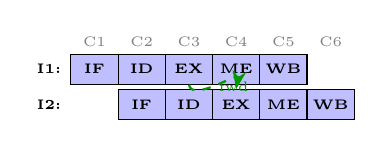
\begin{tikzpicture}
        % Cycle-number header row
        \foreach \idx/\cx in
          {1/0.30, 2/0.90, 3/1.50, 4/2.10, 5/2.70, 6/3.30}{
          \node[font=\tiny, text=gray] at (\cx, 0.80) {C\idx};
        }
        % I1 row
        \node[font=\tiny\bfseries, anchor=east] at (0.00, 0.45) {I1:};
        \node[blk]           at (0.30, 0.45) {IF};
        \node[blk]           at (0.90, 0.45) {ID};
        \node[blk] (i1ex)    at (1.50, 0.45) {EX};
        \node[blk]           at (2.10, 0.45) {ME};
        \node[blk]           at (2.70, 0.45) {WB};
        \node[emp]           at (3.30, 0.45) {};
        % I2 row (no stalls)
        \node[font=\tiny\bfseries, anchor=east] at (0.00, 0.00) {I2:};
        \node[emp]           at (0.30, 0.00) {};
        \node[blk]           at (0.90, 0.00) {IF};
        \node[blk]           at (1.50, 0.00) {ID};
        \node[blk] (i2ex)    at (2.10, 0.00) {EX};
        \node[blk]           at (2.70, 0.00) {ME};
        \node[blk]           at (3.30, 0.00) {WB};
        % Forwarding bypass: EX result of I1 → EX input of I2
        \draw[fwdarr] (i1ex.south)
          to[out=-80, in=80]
          node[right, font=\tiny, green!60!black, inner sep=1pt] {fwd}
          (i2ex.north);
      \end{tikzpicture}
      \end{center}
      \centering{\scriptsize \textcolor{green!60!black}{0 stalls} $\Rightarrow$ \textbf{6 total cycles}}
    \end{column}

  \end{columns}

  % ── Step-by-step tabular ────────────────────────────────────────────────
  \smallskip
  {\scriptsize\textbf{Step-by-step table (no forwarding vs.\ forwarding):}}
  \begin{center}
  {\scriptsize\setlength{\tabcolsep}{3.5pt}
  \begin{tabular}{l|cccccccc}
    \hline
    Instruction & C1 & C2 & C3 & C4 & C5 & C6 & C7 & C8 \\
    \hline
    I1 (ADD R1,R2,R3)   & IF & ID & EX & ME & WB &    &    &    \\
    I2 without fwd      &    & IF & ID & \textcolor{red}{--} & \textcolor{red}{--} & EX & ME & WB \\
    I2 with fwd         &    & IF & ID & EX & ME & WB &    &    \\
    \hline
  \end{tabular}}
  \end{center}

  {\scriptsize
  \textbf{Result:} Without forwarding: \textbf{2 stalls} (8 cycles).
  With forwarding: \textbf{0 stalls} (6 cycles) --- \textbf{25\% speedup}.}
\end{frame}

% ═════════════════════════════════════════════════════════════════════════════
% Slide 7 — Structural Hazards  [v2 — unchanged]
% ═════════════════════════════════════════════════════════════════════════════
\begin{frame}{Structural Hazards}
  \textit{Two delivery trucks arriving at a warehouse with a single loading dock
  at the same time: one must wait. Structural hazards are the same idea ---
  two pipeline stages need the same piece of hardware simultaneously.}

  \medskip
  \begin{itemize}
    \item \textbf{Memory conflict:} If the CPU has only one memory unit (no
          separate instruction cache and data cache), the Fetch stage and the
          Memory stage cannot both run in the same cycle --- one must stall.
    \item \textbf{Register write-port conflict:} A register file with a single
          write port cannot accept two write-back results in the same cycle.
          \textit{One printer, two print jobs queued at the same instant.}
    \item \textbf{Multi-cycle unit contention:} Slow operations (floating-point
          divide, square root) tie up a shared unit for many cycles, blocking
          other instructions from using it.
    \item \textbf{Fixes:} Add duplicate hardware (two memory ports), share the
          resource across alternating cycles, or let the compiler schedule
          independent work in between.
  \end{itemize}
\end{frame}

% ═════════════════════════════════════════════════════════════════════════════
% Slide 8 — Control Hazards  [v2 — unchanged]
% ═════════════════════════════════════════════════════════════════════════════
\begin{frame}{Control Hazards}
  \textit{You are driving and your GPS says ``turn left'' --- but you are
  already in the right lane three blocks back. You have ``fetched'' the wrong
  road. A branch hazard is the same: the CPU grabs the wrong next instructions
  before it knows which way a branch (an \texttt{if}/\texttt{loop}) goes.}

  \medskip
  \begin{itemize}
    \item A branch's direction and destination are only known at the EX stage,
          so 2 instructions are already fetched for the wrong path --- they must
          be \textbf{flushed} (thrown away), wasting 2 cycles.
    \item \textbf{Static prediction:} Always guess ``branch not taken'' (keep
          driving straight). Simple, but wrong for loops.
    \item \textbf{Dynamic prediction (2-bit counter):} The CPU remembers past
          behaviour in a small table and guesses based on history --- like a GPS
          that learns your usual route.
    \item \textbf{Branch Target Buffer (BTB):} Caches the destination address
          so the CPU can jump immediately without recomputing where to go.
    \item \textbf{Delayed branch:} The slot right after a branch always executes;
          the compiler fills it with a useful instruction instead of wasting it.
  \end{itemize}
\end{frame}

% ═════════════════════════════════════════════════════════════════════════════
% Slide 9 — Hazard Mitigation Summary  [v2 — unchanged]
% ═════════════════════════════════════════════════════════════════════════════
\begin{frame}{Hazard Mitigation Summary}
  \textit{A factory supervisor has three tools: a stop button (stall), a
  conveyor shortcut (forwarding), and a smart pre-planned schedule (compiler
  reordering). Together they keep the assembly line moving even when hiccups
  occur.}

  \medskip
  \begin{itemize}
    \item \textbf{Stall:} Pause the front of the pipeline and insert an empty
          ``bubble'' instruction --- buys time for the slow stage to finish,
          but costs cycles.
    \item \textbf{Forwarding:} A hardware shortcut that hands a result directly
          from one stage to the next instruction's input, cutting most RAW stalls
          to zero extra cycles.
    \item \textbf{Load-use stall:} The one case forwarding cannot fully fix; a
          single wasted cycle is unavoidable unless the compiler reorders code.
    \item \textbf{Branch delay slot:} The instruction after a branch always
          runs; filling it with real work (not a \texttt{NOP}) recovers a cycle
          for free.
    \item \textbf{Compiler scheduling:} By rearranging independent instructions
          at compile time, the compiler can eliminate many hazards before the
          hardware ever sees them.
  \end{itemize}
\end{frame}

% ═════════════════════════════════════════════════════════════════════════════
% Slide 10 — References  [v2 — unchanged]
% ═════════════════════════════════════════════════════════════════════════════
\begin{frame}{References}
  \begin{thebibliography}{9}
    \bibitem{patterson} Patterson, D.\,A. and Hennessy, J.\,L.
      \textit{Computer Organization and Design: The Hardware/Software Interface},
      5th ed. Morgan Kaufmann, 2014.
    \bibitem{hennessy} Hennessy, J.\,L. and Patterson, D.\,A.
      \textit{Computer Architecture: A Quantitative Approach},
      6th ed. Morgan Kaufmann, 2017.
  \end{thebibliography}
\end{frame}

\end{document}
